\chapter{REVISIÓN DE LITERATURA}


  % o	Ciencia ciudadana
  % Es una forma de investigación colaborativa que involucra a todas las personas interesadas en participar, con la finalidad de aprender sobre un tema y solucionar problemas juntos.
  % o	Precipitación
  % Es la caída de agua procedente de las nubes en estado líquido (lluvia y llovizna),  sólido (granizo) y semisólido (nieve). Es una parte importante de ciclo hidrológico, ya que sin la precipitación no habría agua en los ecosistemas, ni en los lugares en donde vivimos.
  % o	Monitoreo
  % Consiste en la observación de un suceso o fenómeno para recolectar información bajo un método previamente establecido. En el caso del monitoreo de la precipitación, se refiere al registro de los niveles de agua almacenados en los pluviómetros.
  % o	Pluviómetro
  % Es un dispositivo diseñado para almacenar el agua procedente de la precipitación que cae en una superficie y tiempo determinado.



\section{Definición de términos clave}
En un sistemas meteorológico a pequeña escala, donde participa la formación de nubes del tipo cúmulus dependiendo la presencia de núcleos de condensación; Temperaturas cercanas a la del punto de rocío; Abasto continuo de vapor de agua; Incremento del tamaño de las gotas a través de colisiones; se pueden presentar diferentes fenómenos meteorológicos tales como la lluvia, el granizo, la nieve, las trombas, los tornados, los rayos y los truenos.
\begin{definition}[Precipitación]
  Es la caída de agua procedente de las nubes en estado líquido, sólido y semisólido (\cite{breña2013}).
\end{definition}


El monitoreo es fundamental para la toma de decisiones informadas en la gestión ambiental y otros campos.
\begin{definition}[Monitoreo]
  Es un proceso sistemático y continuo que permite observar, registrar y analizar parámetros específicos para evaluar el estado o cambios en un sistema o fenómeno determinado.(\cite{ciga_monitoreo})
\end{definition}


\begin{definition}[Ciencia Ciudadana]
Es una metodología científica que involucra activamente a la ciudadanía en la generación de conocimiento, permitiendo que personas sin formación científica formal participen en la recolección, análisis e interpretación de datos, contribuyendo así a proyectos de investigación y al fomento de la cultura científica.(\cite{csic_ciencia_ciudadana})
\end{definition}


\begin{definition}[Flutter]
Flutter es un framework de código abierto desarrollado por Google que permite crear aplicaciones nativas de alto rendimiento para múltiples plataformas (iOS, Android, web, escritorio) a partir de una única base de código, utilizando el lenguaje de programación Dart.(\cite{flutter_multiplataforma})
\end{definition}

\begin{definition}[Dart]

Dart es un lenguaje de programación desarrollado por Google, diseñado para crear aplicaciones frontend rápidas y optimizadas, especialmente utilizado en conjunto con Flutter. (\cite{dart})
\end{definition}
\begin{definition}[Firebase]

Firebase es una plataforma de desarrollo de aplicaciones creada por Google que proporciona servicios como bases de datos en tiempo real, autenticación de usuarios, hosting de archivos y funciones de backend sin servidor, facilitando el desarrollo y escalamiento de aplicaciones móviles y web. (\cite{firebase})
\end{definition}


\begin{definition}[Backend]
El backend se refiere a la parte del desarrollo de software que gestiona la lógica de negocio, bases de datos, servidores y APIs, funcionando como la estructura interna que sostiene y conecta los servicios de una aplicación.(\cite{backend})
\end{definition}



\begin{definition}[Frontend]
  El frontend es la capa de una aplicación que interactúa directamente con el usuario, encargándose del diseño, la estructura y la experiencia visual mediante tecnologías como HTML, CSS y JavaScript o frameworks como Flutter para móviles.(\cite{frontend})
\end{definition}




\begin{definition}[Google Play Console]
  Google Play Console es la plataforma de gestión que permite a los desarrolladores publicar, actualizar, monitorear el rendimiento y administrar la distribución de sus aplicaciones Android en la tienda Google Play.(\cite{googleplayconsole})


\end{definition}

\begin{definition}[Firebase Realtime Database]
Es un servicio de base de datos en la nube que almacena y sincroniza datos entre usuarios en tiempo real, ideal para aplicaciones que requieren actualizaciones inmediatas. (\cite{firebaserealtime})
\end{definition}
















\begin{definition}[Pluviómetro manual]

El pluviómetro manual es un instrumento utilizado para medir la cantidad de precipitación líquida caída en un lugar específico durante un período determinado. Consiste en un recipiente cilíndrico que recoge el agua de lluvia, la cual se mide posteriormente con una probeta graduada. Este instrumento debe cumplir con las especificaciones establecidas en las normas mexicanas para garantizar la precisión y confiabilidad de los datos obtenidos.(\cite{semarnat_pluviometro})
\end{definition}

Las especificaciones para construir un pluviómetro, ilustradas en la figura \ref{t1}, son las siguientes:
\begin{itemize}
    \item El depósito debe tener una entrada estrecha, suficientemente protegida de la radiación, para reducir al mínimo las pérdidas de agua por evaporación
    \item Este instrumento debe colocarse en lugares abiertos y su área de captación debe permanecer horizontal y a 100 cm del suelo. (\cite{se2013})
\end{itemize}

\begin{figure}[ht]
\centering
  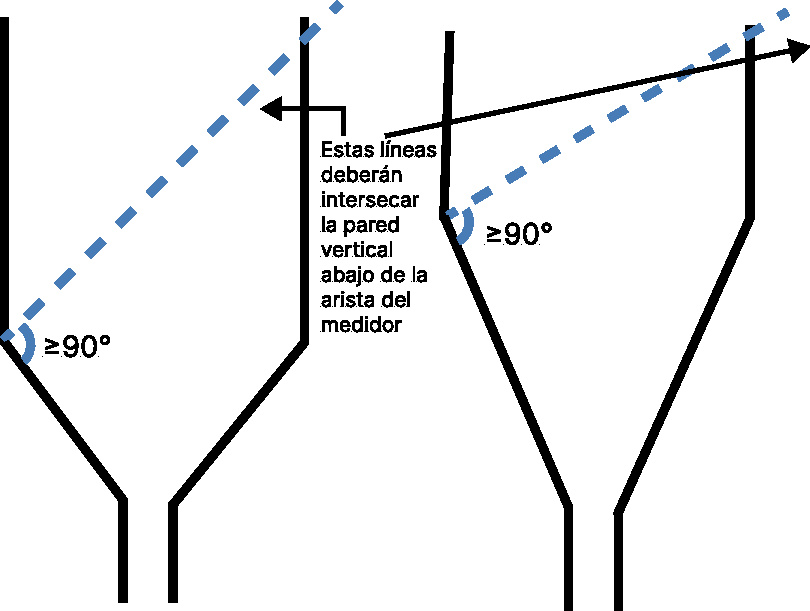
\includegraphics[width=0.5\textwidth]{t1.pdf}
  \caption{Colectaros adecuados para los pluviómetros según la norma NMX-AA-166/1-SCFI-2013 (\cite{se2013})}
  \label{t1}
\end{figure}




















\section{Acceso a datos meteorológicos de zonas de montaña en México}
% TODO
















\section{Revisión de estudios previos sobre monitoreo ciudadano meteorológico}

Un artículo publicado en RMetS por Samuel Michael Illingworth et al., titulado “Red de ciudadanos sobre precipitaciones del Reino Unido: un estudio piloto”, describe cómo se utilizó GoogleChart para llevar un registro colaborativo de las precipitaciones.(\cite{illingworth2021ukprecipitation}) 

Por otro lado, el artículo “Enhancing Engagement of Citizen Scientists to Monitor Precipitation Phase” menciona la aplicación Mountain Rain or Snow, una colaboración financiada por la NASA entre Lynker, Desert Research Institute y la Universidad de Nevada-Reno. Esta aplicación permite a los usuarios reportar si está lloviendo o nevando en un momento y lugar determinados.(\cite{lute2021enhancing})


En el contexto de África, el artículo “Evaluation of Factors Affecting the Quality of Citizen Science Rainfall Data in Akaki Catchment, Addis Ababa, Ethiopia” aborda los factores que influyen en la calidad de los datos sobre precipitaciones recolectados por científicos ciudadanos.(\cite{tedla2022evaluation}) 

Asimismo, la aplicación iFlood, mencionada en el estudio “Coastal Flooding Generated by Ocean Wave- and Surge-Driven Groundwater Fluctuations on a Sandy Barrier Island”, tiene un enfoque similar, pero está diseñada específicamente para reportar inundaciones.(\cite{elgar2021coastal}) 


Otras iniciativas destacan el uso de la ciencia ciudadana para monitorear la calidad del agua y llenar vacíos de datos para cumplir con los Objetivos de Desarrollo Sostenible de las Naciones Unidas, como se describe en el artículo “Using Citizen Science to Understand River Water Quality While Filling Data Gaps to Meet United Nations Sustainable Development Goal 6 Objectives”.(\cite{mcginn2021using})

En un enfoque relacionado, el desarrollo de aplicaciones móviles para el monitoreo de aguas subterráneas también ha sido promovido como una herramienta para involucrar a la ciencia ciudadana, según se menciona en el estudio “Groundwater Mobile App Development to Engage Citizen Science”.(\cite{dennis2019groundwater})



véase la figura 2 para ubicar sus categorías.














\section{Tecnologías actuales en monitoreo climático}
La implementación de herramientas tecnológicas para el monitoreo de fenómenos climáticos ha demostrado ser una estrategia eficiente, especialmente cuando se combina con enfoques de ciencia ciudadana. Este estudio, al fomentar la colaboración comunitaria y el uso de tecnologías accesibles, tiene el potencial de generar información crítica para el manejo de los ecosistemas de montaña.

\subsection{Pluviómetros con IoT}

\subsection{Estaciones meteorológicas}














\subsection{Aplicaciones móviles}

Entre los avances más destacados está el proyecto Cooperative Open Online Landslide Repository (COOLR), que utiliza las aplicaciones \textbf{Landslide Reporter} y \textbf{Landslide Viewer}. Estas herramientas invitan a científicos ciudadanos de todo el mundo a contribuir con reportes de eventos de deslizamientos de tierra, mejorando la investigación y predicción de desastres.\cite{coolr2021} 

Además, la aplicación \textbf{Sense-it} ofrece un kit de herramientas de sensores para la investigación ciudadana, funcionando como una herramienta educativa en dispositivos Android.\cite{van2017senseit}


Otra categoría importante son los diarios de lluvia, como la aplicación \textbf{Rain Tracker} de Callum Hill, que permite a los usuarios gestionar sus propios datos de precipitaciones, aunque estos no son accesibles al público. \cite{hill2021raintracker}

Aplicaciones similares encontradas en el mercado de aplicaciones a junio de 2025, como \textbf{Pocket Rain Gauge}, \textbf{Rainlogger} y \textbf{Rain Recorder} registran las precipitaciones en función de la ubicación mediante GPS, pero tampoco ofrecen un sistema de registro público de los datos.


\subsection{Importancia hidrológica de las zonas de montaña}


\section{Aportes del monitoreo ciudadano a la ciencia climática}







